\documentclass{ctexart}
\usepackage{graphicx, longtable, multirow}
\title{数据结构第一次作业}
\author{邵志豪}
\date{March 7, 2023}
\begin{document}
	\maketitle
	\newpage
	\begin{description}
		\item[1.8] 试确定各程序段中@标记语句的频度:
		\begin{description}
			\item[(1)] $n-1$
			\item[(2)] $n-1$
			\item[(3)] $n-1$
			\item[(4)] $\frac{(n+1)n}{2}$
			\item[(5)] $\frac{n(n+1)(n+2)}{6}$
			\item[(6)] $n$
			\item[(7)] $\lfloor \sqrt{n} \rfloor$
			\item[(8)] 1100
		\end{description}
		\item[1.9] $count=\lceil log_2n \rceil-2$,$T(n)=O(log n)$
		\item[1.12] 判断是否正确:
		\begin{description}
			\item[(1)] 正确
			\item[(2)] 正确
			\item[(3)] 错误
			\item[(4)] 正确
			\item[(5)] 错误
		\end{description}
		\item[2.4] 原状态及结果如下图:
		\begin{center}
			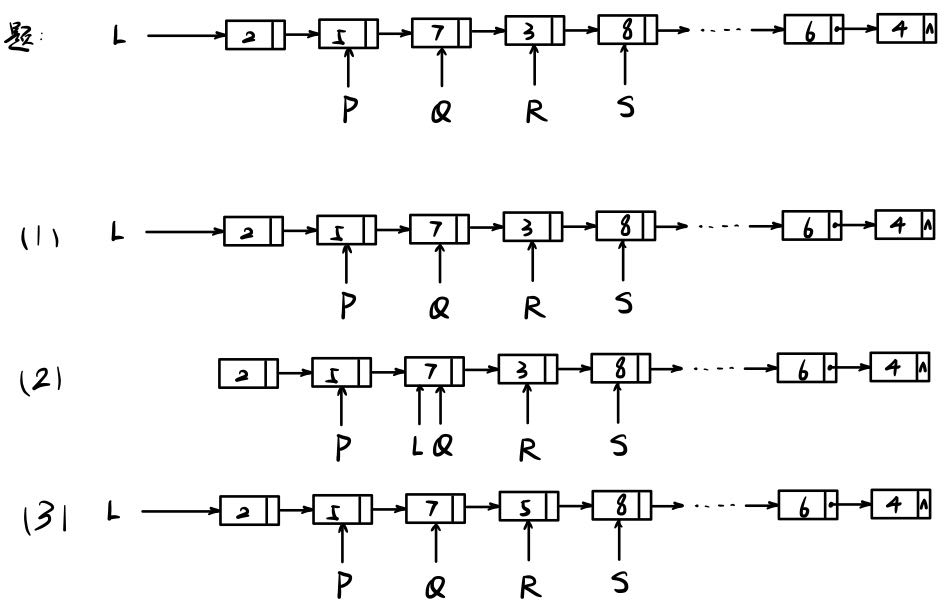
\includegraphics[width=0.9\linewidth]{Pic/2.4.1.jpg}
			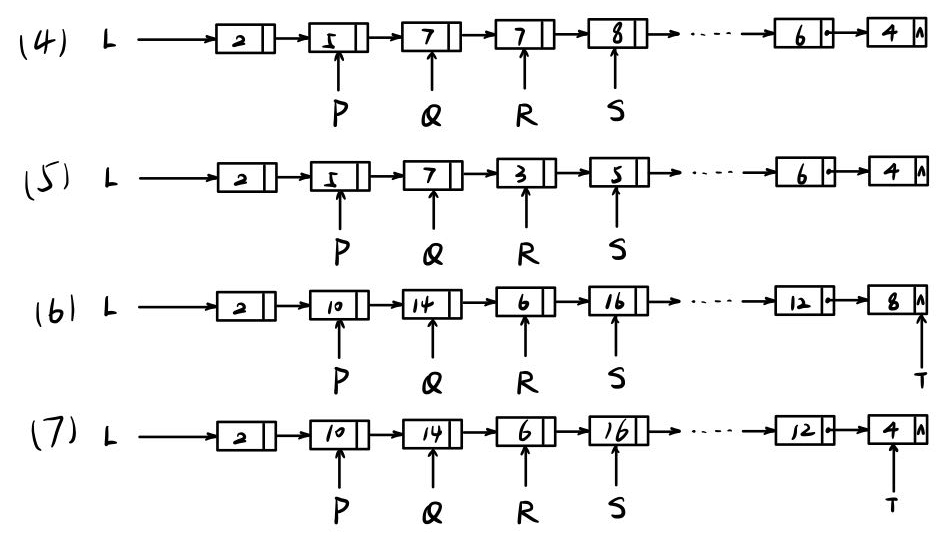
\includegraphics[width=0.9\linewidth]{Pic/2.4.2.jpg}
		\end{center}
		\item[2.5] 各行运行结果如下图:
		\begin{center}
			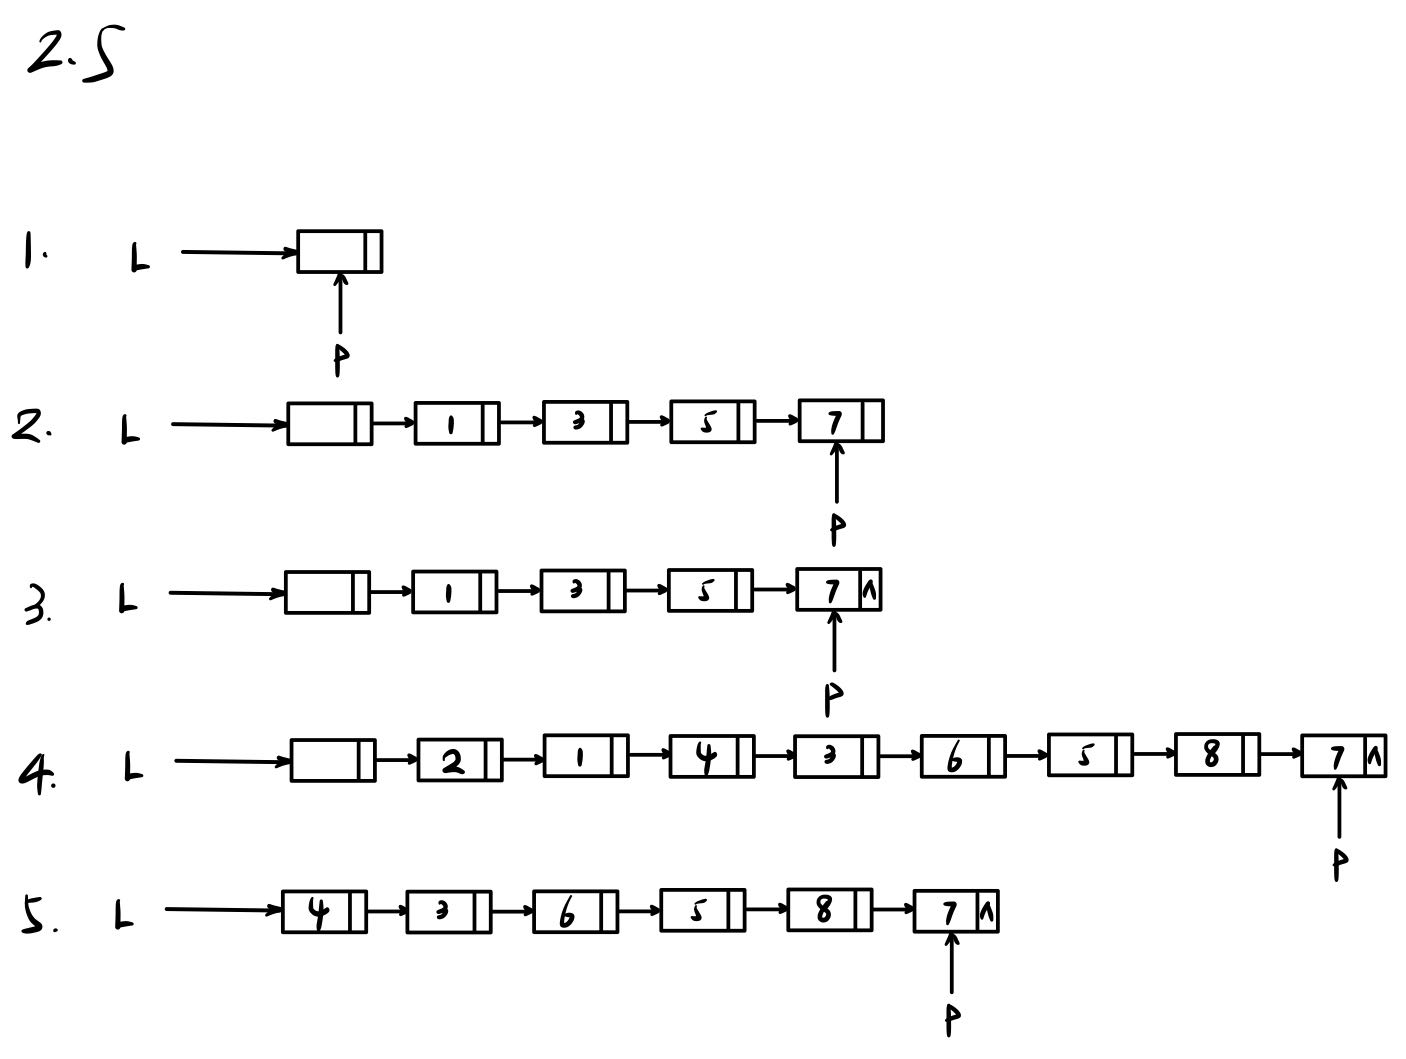
\includegraphics[width=0.9\linewidth]{Pic/2.5.jpg}
		\end{center}
		\item[2.9] 简述以下算法功能:
		\begin{description}
			\item[(1)] 将多数据元素单链表L的第一个数据元素和第二个数据元素接在最后一个数据元素之后,并和第二个数据元素解开链接。
			\item[(2)] 将单循环链表以pa和pb指向的数据元素之前为标记,截断成两段,并各自首尾相连,成为两个单循环链表。
		\end{description}
		\item[3.3] stack
		\item[3.7] 变化过程如下:
		\begin{center}
			\begin{longtable}[c]{c|c|c|c|c}\hline
				步骤&OPTR栈&OPND栈&输入字符&主要操作\\\hline
				1&\#&&\underline{A}-B$\times$C/D+E$\uparrow$F\#&PUSH(OPND,A)\\\hline
				2&\#&A&\underline{-}B$\times$C/D+E$\uparrow$F\#&PUSH(OPTR,'-')\\\hline
				3&\#\quad-&A&\underline{B}$\times$C/D+E$\uparrow$F\#&PUSH(OPND,B)\\\hline
				4&\#\quad-&A\quad B&\underline{$\times$}C/D+E$\uparrow$F\#&PUSH(OPTR,'$\times$')\\\hline
				5&\#\quad-\quad$\times$&A\quad B&\underline{C}/D+E$\uparrow$F\#&PUSH(OPND,C)\\\hline
				6&\#\quad-\quad$\times$&A\quad B\quad C&\underline{/}D+E$\uparrow$F\#&operate(B,'$\times$',C)\\\hline
				7&\#\quad-\quad$\times$&A\quad B$\times$C&\underline{/}D+E$\uparrow$F\#&PUSH(OPTR,'/')\\\hline
				8&\#\quad-\quad/&A\quad B$\times$C&\underline{D}+E$\uparrow$F\#&PUSH(OPND,D)\\\hline
				9&\#\quad-\quad/&A\quad B$\times$C\quad D&\underline{+}E$\uparrow$F\#&operate(B$\times$C,'/',D)\\\hline
				10&\#\quad-&A\quad B$\times$C/D&\underline{+}E$\uparrow$F\#&operate(A,'-',B$\times$C/D)\\\hline
				11&\#&A-B$\times$C/D&\underline{+}E$\uparrow$F\#&PUSH(OPTR,'+')\\\hline
				12&\#\quad+&A-B$\times$C/D&\underline{E}$\uparrow$F\#&PUSH(OPND,E)\\\hline
				13&\#\quad+&A-B$\times$C/D\quad E&\underline{$\uparrow$}F\#&PUSH(OPTR,'$\uparrow$')\\\hline
				14&\#\quad+\quad$\uparrow$&A-B$\times$C/D\quad E&\underline{F}\#&PUSH(OPND,F)\\\hline
				15&\#\quad+\quad$\uparrow$&A-B$\times$C/D\quad E\quad F&\#&operate(E,'$\uparrow$',F)\\\hline
				16&\#\quad+&A-B$\times$C/D\quad E$\uparrow$F&\#&operate(A-B$\times$C/D,'+',E$\uparrow$F)\\\hline
				17&\#&A-B$\times$C/D+E$\uparrow$F&\#&RETURN(GETTOP(OPND))\\\hline
			\end{longtable}
		\end{center}
		\item[3.11] 队列和栈都是操作受限的线性表,他们的数据结构都是线性表,但是他们首先得操作不同:前者要求先进先出,后者要求先进后出;前者要求在线性表的一端插入,另一端删除,后者则只在一端插入和删除;前者遍历时不会影响数据结构,也不会另外开辟空间,后者则需要弹出所需数据之上的所有数据才能遍历,而且需要额外空间进行暂时存储。
	\end{description}
\end{document}